\chapter{Design}
\label{chapter3}
This chapter will outline the proposed design of the cloud gaming system as well as the game that will be used to run on the system. Also at a high level, I will discuss the virtual network design that will be used to simulate a cloud data center as well as the proposed solution to use software-defined networking to reduce latency in the network.

\section{Cloud Gaming System}
As a result of the background research conducted, the cloud gaming system will aim to offload the game engine to the cloud data center. This includes the game logic, physics and graphics rendering. Due to this, it will leave the client's application to just take control of receiving physical button input and send this to the game server as well as receiving and displaying the game video frames.
\newline
\par
It can be seen at Figure \ref{fig:cloudmodel} that multiple players should be able to connect to the cloud server and a new virtual machine should be generated for each player. For each virtual machine, an instance of the game will be executed with the required resources such as RAM and processing power provided by the cloud's resource manager. The resources required can be specified as a template with the parameters already set. This makes sure that each game instance has sufficient resources to run at smoothly.
\newline
\par
A design improvement on this is to allow the client to specify the video settings to use such as 1080p resolution at 60 fames-per-second and 720p resolution at 30 frames-per-second. Enabling this option will give the client an option to manually improve their gameplay experience since sending higher resolution frames as well as more of them per second will require higher bandwidth. This also helps the cloud data centre to use different templates for virtual machine resources so they will not be wasted by providing too much and therefore can be allocated to other virtual machines.
\newline
\par
The software-defined networking controller will manage the networking inside the data centre. It will have global knowledge of the all switches and the links between them. A load balancing application will be used to make sure that traffic generated with the video streaming is routed appropriately to help keep latency in the network to a minimum. This will be discussed later on section 3.4.
\clearpage
\begin{figure}[h!]
 \centering
 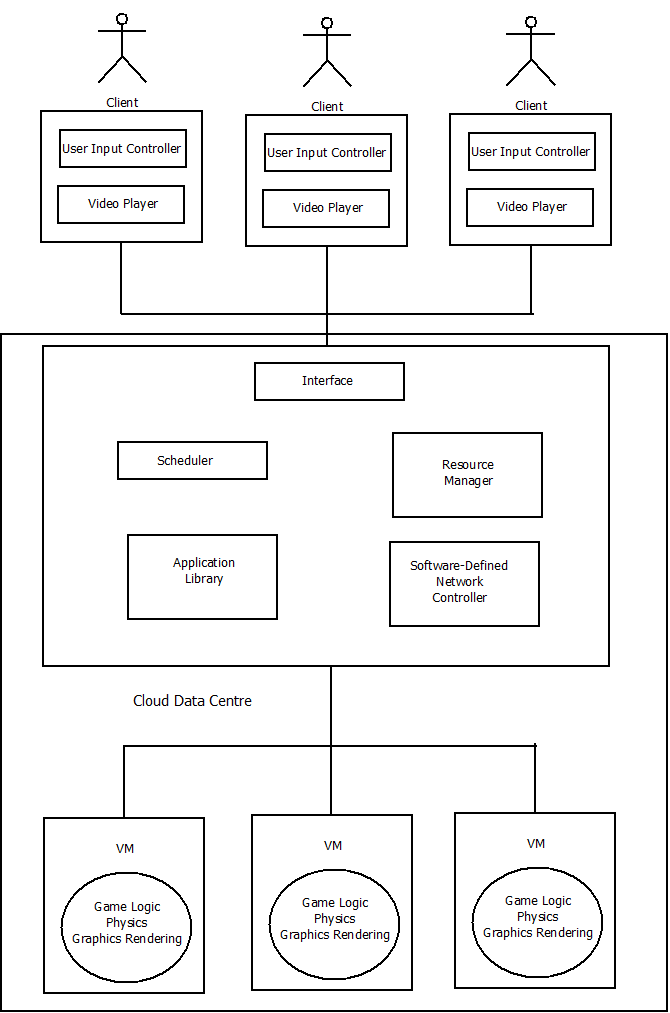
\includegraphics[width=0.9\linewidth]{images/cloudsystemmodel.png}
 \caption{Cloud Gaming System Model}
 \label{fig:cloudmodel}
\end{figure}

\section{Game Design}
In this section I will indicate the design of the game at a high level that will developed to be used as the program to benchmark on the cloud gaming system. The aim of this game is to be somewhat computationally expensive to warrant as a program that will improve by being on a system that is more powerful than a mainstream consumer system. The game should be configurable so it can test out the limits of the system by increasing the amount of computer power it needs. It should also implement a method to measure latency that will arise not just numerically but through user input and immediate visual feedback. The client will experience this lag when a button is pressed, but the expected visual feedback is not being displayed as soon as expected.
\newline
\par
To make the game computationally challenging, trees will be modelled and generated in real time. Plants and trees are part of the natural environment and are often used in games to create a realistic scenery. They are geometrically complex and difficult to generate realistic models in real time. Such trees are usually pre-generated and saved locally so it can be loaded easily when needed, but this means the game is limited to using those models and tree models will have to be repeated. This degrades the player's experience as they see duplicate trees in the scenery reminding them that they are in a game which breaks the immersion.
\newline
\par
Lindenmayer systems or 'L-systems' is a part of formal language theory to write parallel grammars describing growth similar to the way DNA is a programming language of the human body \cite{prusinkiewicz2012algorithmic}. Plants tend to have patterns in their growth, but fundamentally they grow forward, rotate then branch out in a hierarchy starting from the root. L-systems are stated as production rules and correspond to each stage of growth for each part of the plant according to a fixed pattern. The notation in the pattern can be simplified to:
\begin{itemize}
 \item F 	:	move forward and draw
 \item +,- \(\theta\)	:	rotate \(\theta\) around x-axis
 \item \&,\(\wedge\) \(\theta\)	:	rotate \(\theta\) around y-axis
 \item /,\(\backslash\) \(\theta\)	:	rotate \(\theta\) around z-axis
 \item {[,]}	:	push / pop
\end{itemize}

Using the symbols above, grammars for tree generation can be produced that will specify the pattern to be followed. The symbols '[' and ']'  which represent push and pop respectively refer to a Last in First Out stack. When the symbol '[' is reached, the current position and angle is saved and are restored when the symbol ']' is encountered. Variations can be implemented through randomized parameters such as random angles for rotation and length of branches. For more complex games, environmental factors can be used to determine the parameters such as competition for light, food, diseases and animals \cite{plantslecture}. For the game produced from this project, random rotation angles will be used to generate variation. The production rules below are recursive and will produce two branches for each branch on each recursion.

\[Trunk \rightarrow F[+\theta /\theta Branch][-\theta \backslash\theta Branch]\]
\[Branch \rightarrow F[+\theta /\theta Branch][-\theta \backslash\theta Branch]\]

To better illustrate how a tree is produced at each recursion, Figure \ref{fig:tree} shows a two dimensional version. The production rules are based on the Pythagoras tree which is a tree constructed from squares and is named due to each triple of squares enclose a right angle triangle. The tree starts with one square and with each recursion two squares are used for each square from the previous recursion. As shown in Figure \ref{fig:tree}, the amount of branches grows in size and complexity pretty quickly, in fact it grows exponentially where the total branches equal to \(2^n - 1\) with n being the number of recursions.

\begin{figure}[h!]
 \centering
 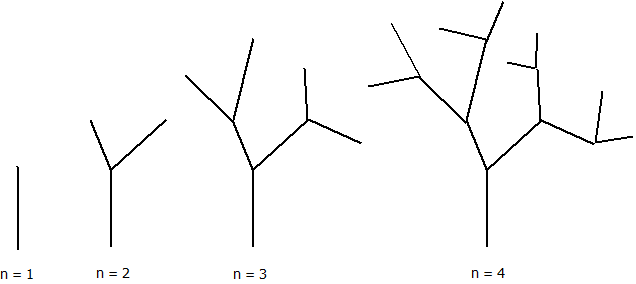
\includegraphics[width=0.8\linewidth]{images/tree.png}
 \caption{2D Pythagorean L-system tree}
 \label{fig:tree}
\end{figure}

Computing the vertices of these many branches in real time will be expensive and adding lighting and shadows will add even more to the resource requirement. Projective shadows is a shadow technique that casts shadows by point light sources onto planes. It takes advantage of a shadow matrix that uses persepective transformation to render an object on to the plane depending on the position of the light source \cite{hawkins2001opengl}. The problem with this is that it doubles the computation since the object is being rendered twice; the actual object and its shadow. To measure the performance, a frames-per-second counter should be used. The higher the number the FPS counter shows, it means the higher performance the system is capable of since it can push more frames at a given time which means the player will have a smoother gameplay experience. An important factor that should also 
\newline
\par
In order for latency to be evident when playing the game, a form of interaction needs to implemented. A simple flight simulator was chosen so the user can traverse the game and be a way to view the tree model from different angles. The flight simulator will support basic controls such as acceleration and deceleration and roll, yaw and pitch movement. Latency will be easily detected when the user inputs a command then the game's camera doesn't move immediately.

\section{Virtual Network}
Due to limitations with the School of Computing cloud testbed, the proposed solution of software-defined networking to mitigate latency will not be able to be conducted. An alternative solution is to simulate the video traffic that would have been using the data centre's network. This can be done through virtual networks where it can run real kernel, switch and application code on a single machine. Simulating a network also means that switched and links can be easily configurable for software-defined networking controller to work and to simulate real world factors such as latency and bandwidth limitations.

\begin{figure}[h]
 \centering
 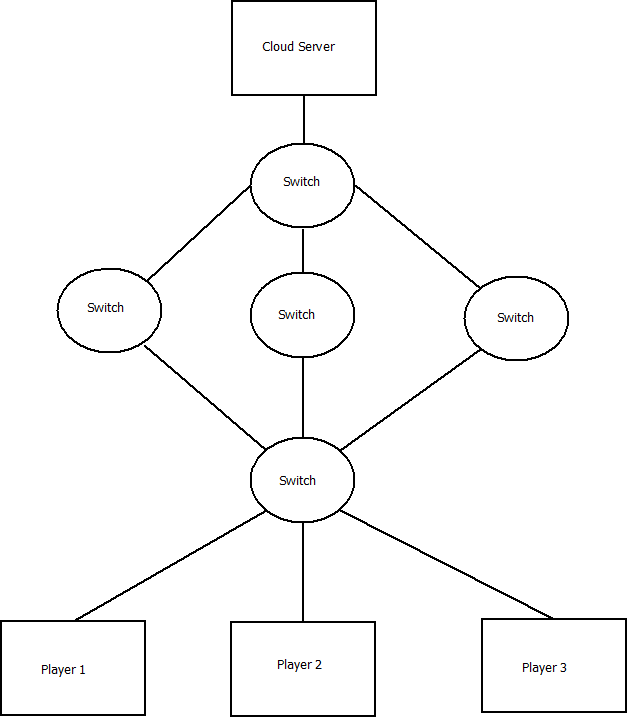
\includegraphics[width=0.7\linewidth]{images/network.png}
 \caption{Virtual Network Topology}
 \label{fig:network}
\end{figure}

\section{SDN Application Design}
\lipsum[1-1]